\subsection{第 5 课 | 哈希表、映射、集合}

\subsubsection{脑图}

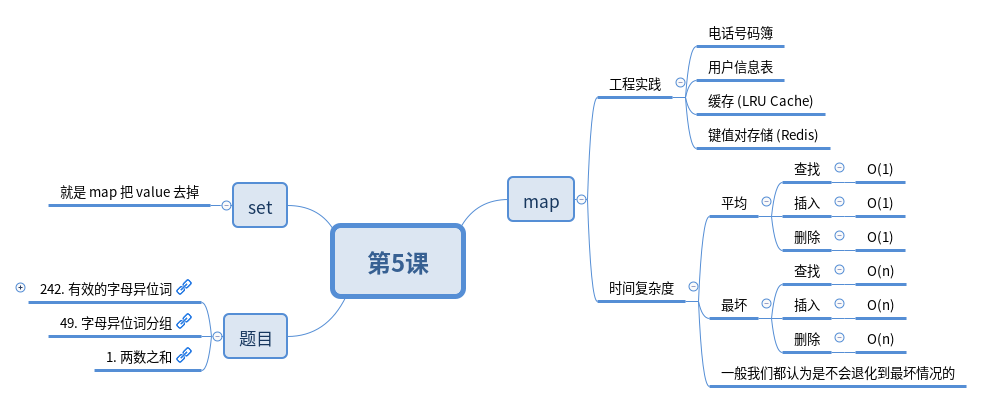
\includegraphics[width=170mm,height=80mm]{images/第5课.png}

\subsubsection{题目}

\begin{itemize}
\item \hyperref[leetcode:242]{242. 有效的字母异位词}
\item \hyperref[leetcode:49]{49. 字母异位词分组}
\item \hyperref[leetcode:1]{1. 两数之和}
\end{itemize}
